Důsledná a přesná specifikace {objektů} a jejich {tříd} v etapě návrhu umožňuje\textbf{ automatické generování zdrojových kódů}. K mapování UML diagramů na kód dochází v první části implementační fáze vývoje.

Z \textbf{diagramu tříd} lze vygenerovat jednotlivá rozhraní, třídy s proměnnými a metodami (bez implementace) - \url{http://www.milosnemec.cz/clanek.php?id=199}. Úkolem samotné implementace je pak dopsat těla metod, jejichž chování může být popsáno v \textbf{diagramu aktivit}.

\begin{table}[H]
	\centering
	\begin{tabular}{|l|l|}
		\hline
		\textbf{Analýza a návrh (UML)} & \textbf{Zdrojový kód (Java)}                                \\ \hline
		Třída                          & Struktura typu class                                        \\ \hline
		Role, Typ a Rozhraní           & Struktura typu interface                                    \\ \hline
		Operace                        & Metoda                                                      \\ \hline
		Atribut třídy                  & Statická proměnná označená static                           \\ \hline
		Atribut                        & Instanční proměnná                                          \\ \hline
		Asociace                       & Instanční proměnná                                          \\ \hline
		Závislost                      & Lokální proměnná, argument nebo návratová hodnota zprávy    \\ \hline
		Interakce mezi objekty         & Volání metod                                                \\ \hline
		Případ užití                   & Sekvence volání metod                                       \\ \hline
		Balíček, Subsystém             & Kód nacházející se v adresáři specifikovaném pomocí package \\ \hline
	\end{tabular}
\end{table}

Cílem implementace je \textbf{doplnit} navrženou architekturu (kostru) aplikace \textbf{o programový kód} a vytvořit tak kompletní systém.

\textbf{Implementační model }specifikuje, jak jsou jednotlivé elementy (objekty a třídy) implementovány ve smyslu softwarových komponent.

\textbf{Softwarová komponenta} je definována jako \textbf{fyzicky existující} a \textbf{zaměnitelná část} systému, která vyhovuje požadované množině rozhraní a poskytuje jejich realizaci. Typy softwarových komponent dělíme na:

\begin{itemize}
\item \textbf{Zdrojové kódy} - části systému zapsané v programovacím jazyce.
\item \textbf{Binární a spustitelné kódy} - přeložené do strojové kódu procesoru.
\item \textbf{Ostatní části} - databázové tabulky, dokumenty apod.
\end{itemize}

Jestliže jsme ve fázi analýzy a návrhu pracovali pouze s abstrakcemi dokumentovanými v podobě jednotlivých {diagramů}, pak v \textbf{průběhu implementace dochází k jejich fyzické realizaci}. Implementační model se tedy také zaměřuje na specifikaci toho, jak budou tyto {komponenty fyzicky organizovány podle implementačního prostředí}, pro splnění těchto cílů lze využít následující diagramy:
\begin{itemize}
\item \textbf{Diagram komponent} - ilustruje organizaci a závislosti mezi softwarovými komponentami.
\item \textbf{Diagram nasazení} - upřesňuje nejen konfiguraci technických prostředků, ale především rozmístění implementovaných softwarových komponent na těchto prostředcích.
\end{itemize}

\begin{figure}[H]
	\centering
	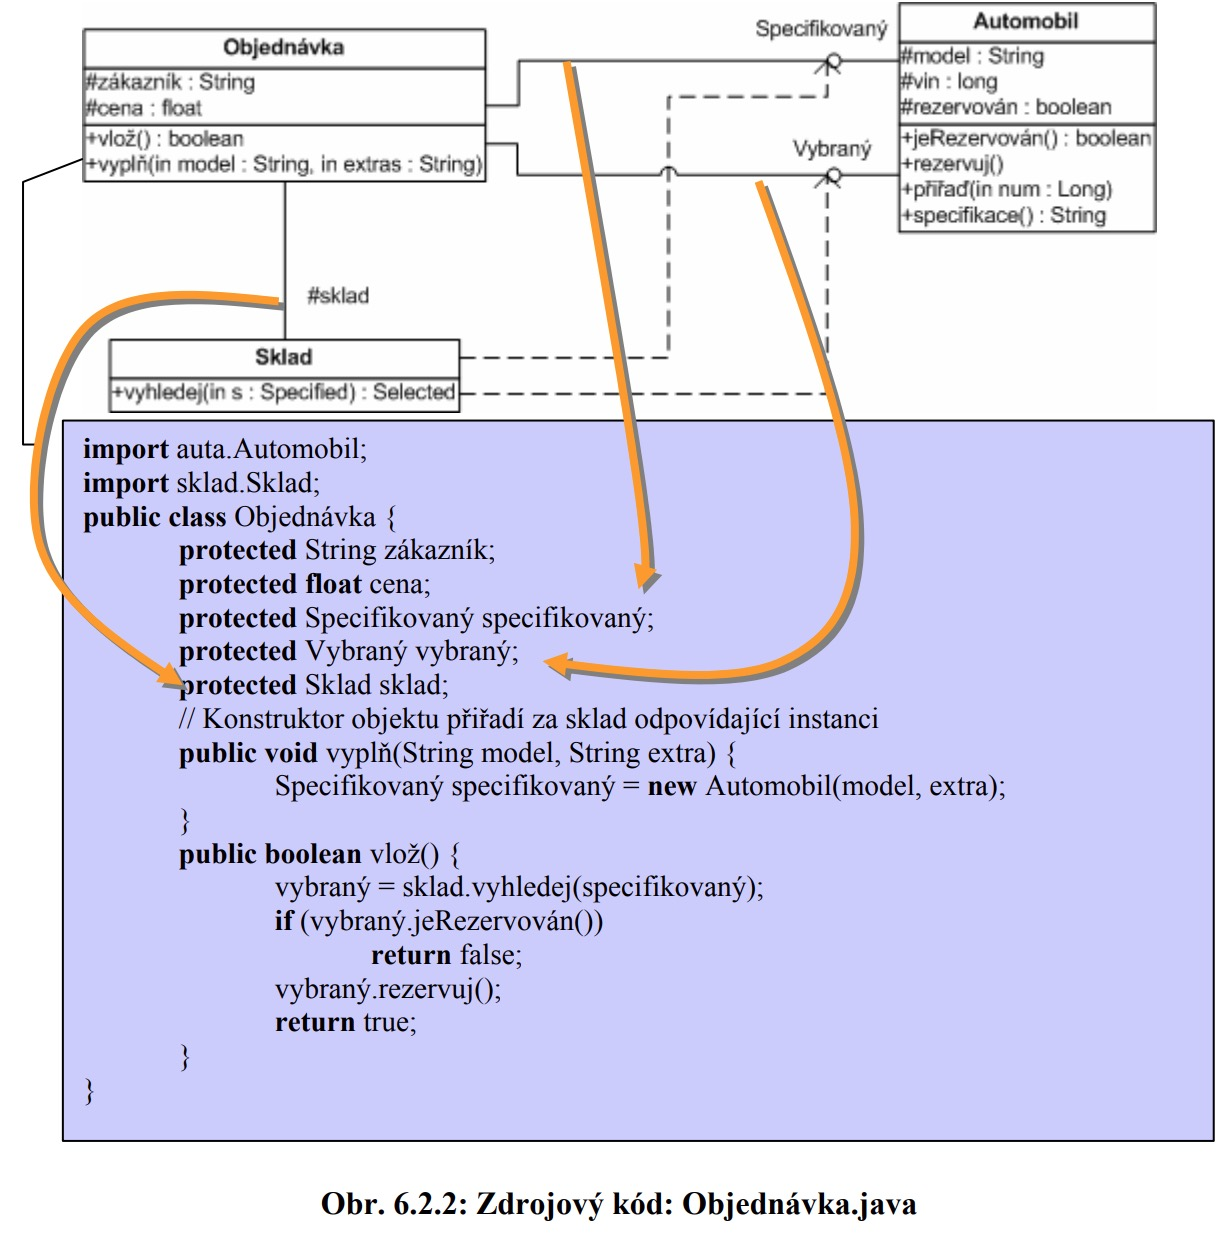
\includegraphics[width=.8\textwidth]{assets/mapovani_uml.jpg}
\end{figure}

\begin{figure}[H]
\centering
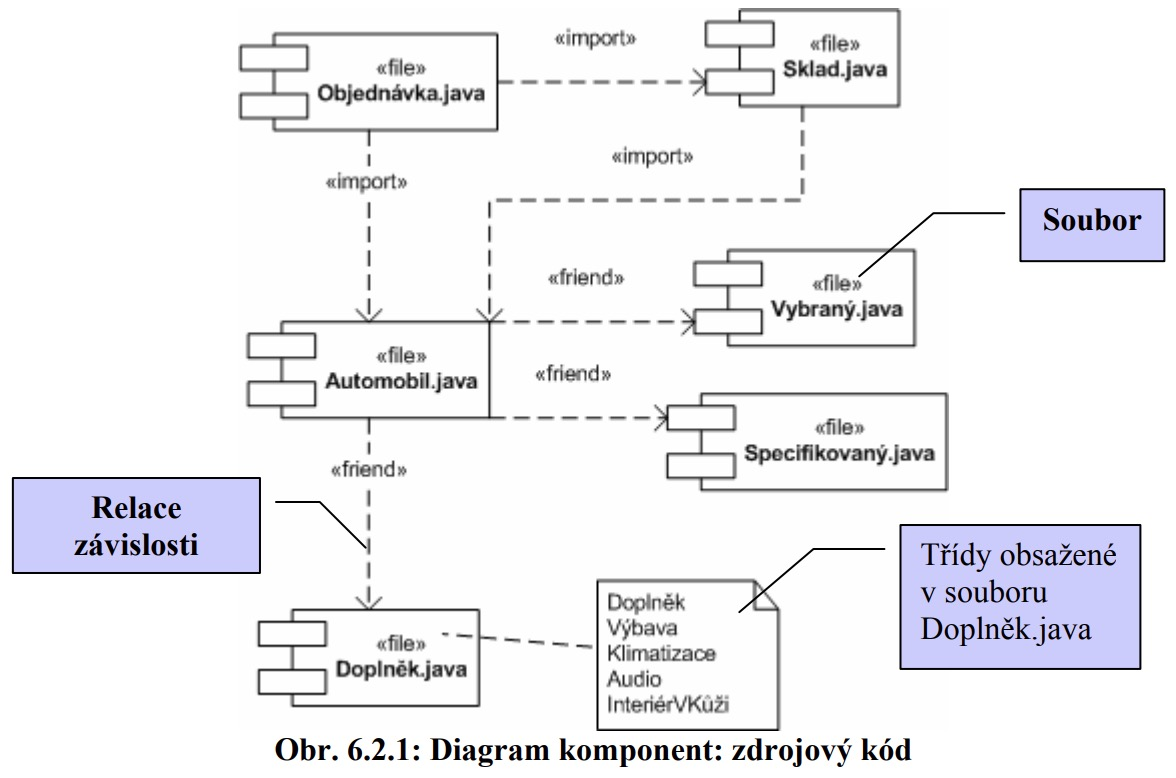
\includegraphics[width=.8\textwidth]{assets/diagram_komponent.jpg}
\end{figure}